\chapter{Dados e existência do prêmio}
\label{chap:dados}

Este capítulo descreve as bases de dados utilizadas na dissertação, testa a
existência do prêmio de risco de volatilidade do Bitcoin (H1) e apresenta uma
análise exploratória das principais variáveis de interesse. O objetivo é
caracterizar as propriedades estatísticas do prêmio, bem como sua relação
preliminar com medidas de volatilidade e retornos do ativo, fornecendo
motivação empírica para as análises econométricas e preditivas desenvolvidas
nos capítulos subsequentes.

Com exceção do teste de H1, a análise conduzida neste capítulo possui caráter
estritamente descritivo e exploratório, não implicando inferências causais.
Ainda assim, ela é fundamental para compreender a dinâmica temporal, a
distribuição estatística e a heterogeneidade do prêmio de risco de volatilidade
ao longo da amostra, estabelecendo o pano de fundo empírico para os modelos
apresentados nos Capítulos~\ref{chap:metodologia} e~\ref{chap:retornos_linear}.

A amostra cobre 1.806 observações diárias, de 24 de março de 2021 a 3 de março de 2026.\footnote{A amostra termina em 3 de março de 2026 por construção: o horizonte máximo de previsão avaliado no Capítulo~\ref{chap:retornos_linear} é de 60 dias, e as últimas 60 observações da série não dispõem de retorno futuro válido nesse horizonte. Embora as análises descritivas deste capítulo e a caracterização por regimes do Capítulo~\ref{chap:retornos_nao_linear} não dependam do alvo de 60 dias, a dissertação adota a mesma amostra em todos os capítulos para assegurar comparabilidade entre os resultados.} Os preços diários do Bitcoin vêm da API pública da Binance (par BTCUSDT), e a volatilidade implícita, do índice DVOL da Deribit. A base de preços original não tinha os dias de 1º a 31 de março de 2023; esta dissertação completa o intervalo com as velas diárias da mesma fonte. Sem essa correção, o retorno registrado em 1º de abril de 2023 acumularia 32 dias e inflaria a volatilidade histórica e o prêmio de abril de 2023. O período inclui a aprovação dos ETFs de Bitcoin à vista pela \textit{Securities and Exchange Commission} (SEC), em janeiro de 2024 --- evento institucional cujo potencial efeito estrutural sobre a dinâmica do BVRP o Capítulo~\ref{chap:retornos_nao_linear} discute como limitação.

% =========================================================
\section{Descrição das variáveis e estatísticas descritivas}
\label{sec:dados-descritivas}

A base de dados combina informações diárias do mercado à vista e do mercado de
opções de Bitcoin: (i) log-retornos diários do Bitcoin no mercado à vista;
(ii) a volatilidade histórica (VH) construída a partir desses retornos;
(iii) a volatilidade implícita (IV) extraída das opções negociadas na
plataforma Deribit; e (iv) o prêmio de risco de volatilidade do Bitcoin, nas
duas versões definidas na Seção~\ref{sec:refer-vrp-teorico}: o BVRP,
$\text{VH}_{t+1:t+30} - \text{IV}_t$, e a proxy
$\text{BVRP}^{\text{proxy}}_t = \text{VH}_{t-29:t} - \text{IV}_t$.

As medidas de volatilidade implícita e histórica usam janelas de 30 dias, de
modo a garantir comparabilidade entre ambas, alinhando-se às práticas de
mercado e à literatura empírica sobre prêmio de risco de volatilidade. A
volatilidade implícita a 30 dias é consistente com o horizonte do índice DVOL
da Deribit, e a volatilidade histórica é anualizada considerando a negociação
contínua do mercado de Bitcoin.

A Tabela~\ref{tab:dados-descritivas} apresenta estatísticas descritivas das
principais variáveis empregadas na análise empírica, incluindo média, desvio
padrão, quantis e valores mínimo e máximo. Tanto a volatilidade implícita
quanto a histórica exibem elevada variabilidade, refletindo a natureza
altamente volátil do mercado de criptoativos. O BVRP tem média de
$-8{,}76$ p.p., e a proxy, de $-8{,}63$ p.p., consistente com a existência de
uma compensação paga pelos investidores para se protegerem do risco de
volatilidade no mercado de opções de Bitcoin: a volatilidade implícita supera
a volatilidade histórica dos 30 dias seguintes em 72\% das datas, configurando
um prêmio de seguro. O BVRP é mais disperso que a proxy (desvio padrão de
$17{,}3$ contra $11{,}9$ p.p.), com mínimo de $-75{,}8$ p.p., em novembro de
2022.

\IfFileExists{tables/dados/desc_stats.tex}{
  \begin{table}[H]
\centering
\small
\caption{Estatísticas descritivas das variáveis principais.
Período: mar.\ 2021 -- mar.\ 2026 ($N=1{.}806$ observações diárias).
BVRP e volatilidades em pontos percentuais anualizados;
log-retorno diário em fração decimal.
Curtose reportada como excesso (Fisher): distribuição normal $= 0$.}
\label{tab:dados-descritivas}
\resizebox{\textwidth}{!}{\begin{tabular}{lrrrrrrrrrr}
\toprule
Variável & Média & D.P. & Mín. & p5 & p25 & p75 & p95 & Máx. & Assim. & Curtose \\
\midrule
BVRP (p.p.) & -8,76 & 17,26 & -75,83 & -35,67 & -19,12 & 1,71 & 20,28 & 46,10 & 0,241 & 0,734 \\
BVRP$^{\text{proxy}}$ (p.p.) & -8,63 & 11,92 & -43,28 & -28,22 & -16,25 & -2,20 & 11,71 & 31,66 & 0,383 & 0,674 \\
VH 30d prospectiva (p.p.) & 53,17 & 19,07 & 16,61 & 26,64 & 39,39 & 65,15 & 85,24 & 121,98 & 0,808 & 0,639 \\
VH 30d retrospectiva (p.p.) & 53,30 & 19,08 & 16,61 & 26,64 & 39,39 & 65,29 & 85,24 & 121,98 & 0,785 & 0,606 \\
IV 30d (p.p.) & 61,93 & 18,70 & 32,38 & 37,65 & 48,12 & 75,02 & 94,98 & 156,20 & 0,820 & 0,407 \\
Log-retorno diário & 0,0001 & 0,0296 & -0,1670 & -0,0472 & -0,0132 & 0,0140 & 0,0461 & 0,1353 & -0,253 & 3,862 \\
\bottomrule
\end{tabular}}
\par\smallskip
\footnotesize\textit{Nota}: VH 30d (volatilidade histórica) calculada como raiz da média dos log-retornos diários quadráticos, anualizada ($\times\sqrt{365}$): retrospectiva sobre os retornos de $t-29$ a $t$; prospectiva sobre os retornos de $t+1$ a $t+30$. IV 30d: índice DVOL da Deribit, observado em $t$. BVRP: $\text{VH}_{t+1:t+30} - \text{IV}_t$; $\text{BVRP}^{\text{proxy}}$: $\text{VH}_{t-29:t} - \text{IV}_t$.
\end{table}

}{}
Os testes formais de estacionariedade confirmam que o preço de fechamento do Bitcoin é integrado de primeira ordem I(1), enquanto os log-retornos diários são estacionários I(0). As medidas de volatilidade (VH 30d e IV 30d) e as duas versões do prêmio apresentam resultados inconclusivos --- o ADF rejeita a raiz unitária, mas o KPSS também rejeita a estacionariedade (no BVRP, com valor-$p$ de $0{,}015$) ---, padrão compatível com processos altamente persistentes, seja por longa memória, seja por uma raiz próxima da unitária. Os testes disponíveis não distinguem entre essas alternativas; para os fins desta dissertação, o que importa é a elevada persistência dessas séries, que motiva tanto o tratamento em nível nas especificações econométricas quanto a atenção ao viés de Stambaugh na inferência do Capítulo~\ref{chap:retornos_linear}. A dissertação mantém essas séries em nível (Tabela~\ref{tab:dados-adf-kpss}).

\IfFileExists{tables/dados/adf_kpss_table.tex}{
  \begin{table}[H]
\centering
\small
\caption{Testes de estacionariedade ADF e KPSS --- variáveis principais da dissertação. Hipótese nula do ADF: presença de raiz unitária; hipótese nula do KPSS: estacionariedade. Período: mar.\ 2021 -- mar.\ 2026 ($N = 1{.}806$ observações diárias).}
\label{tab:dados-adf-kpss}
\begin{tabular}{lrrrrl}
\toprule
Variável & \multicolumn{2}{c}{ADF} & \multicolumn{2}{c}{KPSS} & Conclusão \\
\cmidrule(lr){2-3}\cmidrule(lr){4-5}
 & Estat. & $p$-valor & Estat. & $p$-valor & \\
\midrule
Preço (\textit{close}) & $-1{,}06$ & $0{,}730$ & $4{,}30$ & ${\leq}0{,}01$ & I(1) \\
Log-retorno diário & $-7{,}83$ & $< 0{,}001$ & $0{,}22$ & ${\geq}0{,}10$ & I(0) \\
VH 30d prospectiva & $-4{,}50$ & $< 0{,}001$ & $2{,}35$ & ${\leq}0{,}01$ & Longa memória \\
VH 30d retrospectiva & $-4{,}08$ & $0{,}001$ & $2{,}46$ & ${\leq}0{,}01$ & Longa memória \\
IV 30d & $-2{,}72$ & $0{,}071$ & $4{,}41$ & ${\leq}0{,}01$ & Longa memória \\
BVRP & $-7{,}34$ & $< 0{,}001$ & $0{,}68$ & $0{,}015$ & Longa memória \\
BVRP$^{\text{proxy}}$ & $-6{,}65$ & $< 0{,}001$ & $1{,}19$ & ${\leq}0{,}01$ & Longa memória \\
\bottomrule
\end{tabular}
\par\smallskip
\footnotesize\textit{Nota}: ADF com seleção de defasagens por AIC; KPSS com constante e defasagens automáticas. \textit{Longa memória}: ADF rejeita (ou está na fronteira) e KPSS rejeita a estacionariedade.
\end{table}

}{}

A persistência aparece diretamente nas autocorrelações. A autocorrelação de
primeira ordem é de $0{,}96$ no BVRP e de $0{,}94$ na proxy; na defasagem de
30 dias, ela cai para $-0{,}11$ e $0{,}02$, respectivamente. Os insumos do
prêmio são bem mais persistentes: na mesma defasagem, a autocorrelação é de
$0{,}38$ e $0{,}39$ nas volatilidades históricas prospectiva e retrospectiva e
de $0{,}80$ na volatilidade implícita. A diferença $\text{VH} - \text{IV}$
cancela, portanto, boa parte do componente persistente comum às duas séries,
como antecipado na Seção~\ref{sec:refer-vrp-teorico}. No BVRP, a autocorrelação
elevada nas primeiras defasagens é em parte mecânica: alvos de datas vizinhas
compartilham retornos da mesma janela.

% =========================================================
\section{Existência do prêmio}
\label{sec:dados-h1}

A primeira hipótese da dissertação (H1) é que o prêmio é negativo em média,
isto é, que a volatilidade implícita supera, em média, a volatilidade histórica
dos 30 dias seguintes. O teste regride o BVRP numa constante por MQO, com
erro-padrão de Newey--West: núcleo de Bartlett com $h+1 = 31$ defasagens
\citep{newey1987simple}, número que cobre a sobreposição de até 29 dias entre
alvos vizinhos. A média é de $-8{,}76$ p.p., com erro-padrão de $1{,}70$ e
estatística $t$ de $-5{,}15$ (valor-$p$ de $2{,}6 \times 10^{-7}$): o prêmio é
significativamente negativo. Dois testes de robustez confirmam o resultado.
Primeiro, a estatística $t$ fica entre $-8{,}10$ e $-4{,}92$ quando o número de
defasagens vai de 7 --- a regra automática de \citet{newey1994automatic},
padrão do pacote utilizado --- a 90. Segundo, numa amostra sem sobreposição,
com uma observação a cada 30 dias ($N = 61$), a média é de $-10{,}64$ p.p. e a
estatística $t$ simples, de $-4{,}29$; nos 30 pontos de partida possíveis, ela
fica entre $-4{,}55$ e $-3{,}26$. A proxy leva à mesma conclusão (média de
$-8{,}63$ p.p., $t = -7{,}31$).

% =========================================================
\section{Séries temporais}
\label{sec:dados-series}

A análise das séries temporais das variáveis de interesse permite avaliar a
dinâmica da volatilidade e do prêmio de risco ao longo do tempo, bem como
identificar episódios de persistência e mudanças de comportamento associados a
eventos relevantes do mercado de criptoativos. A
Figura~\ref{fig:dados-series} apresenta, em dois painéis com eixo temporal
compartilhado, a evolução da volatilidade histórica de 30 dias, nas janelas
retrospectiva e prospectiva, e da volatilidade implícita (painel superior) e
das duas versões do prêmio de risco de volatilidade do Bitcoin (painel
inferior), com anotações dos principais eventos de mercado do período.

\IfFileExists{figs/dados/vrp_timeseries.png}{
\begin{figure}[H]
    \centering
    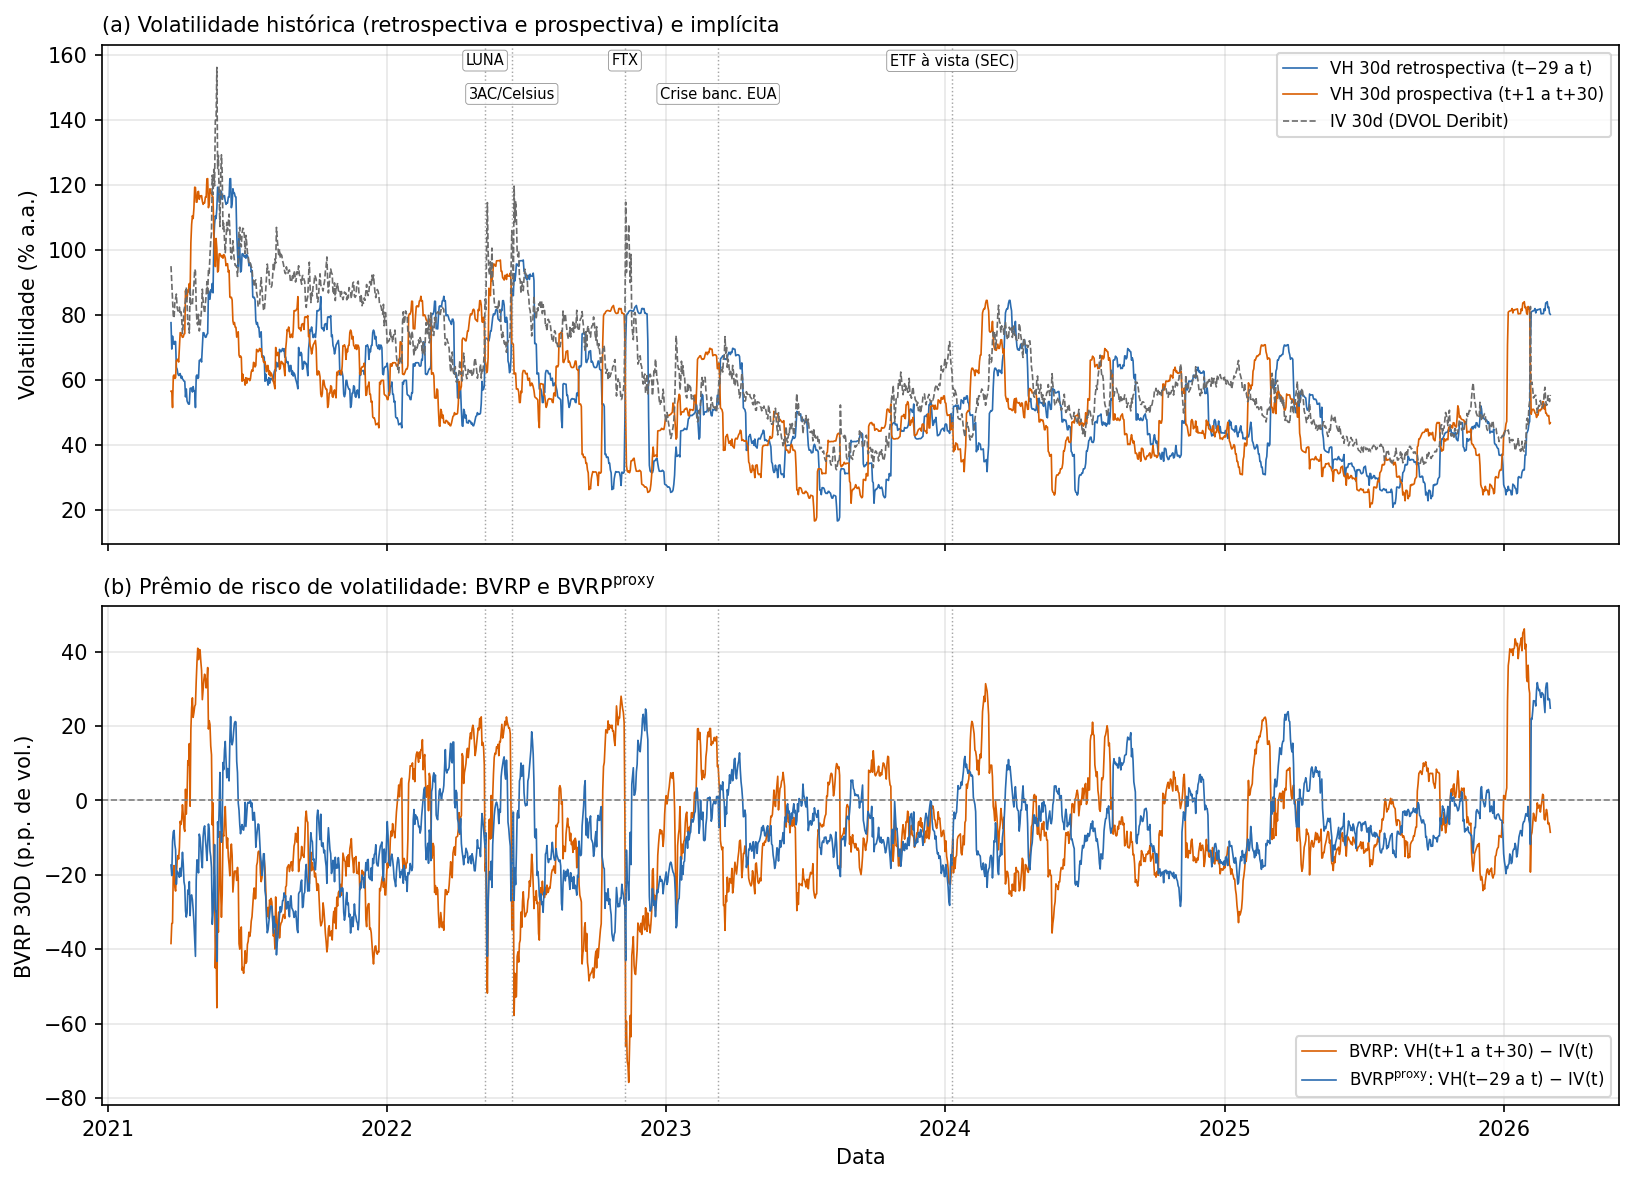
\includegraphics[width=0.9\linewidth]{figs/dados/vrp_timeseries.png}
    \caption{Evolução temporal das séries de volatilidade do Bitcoin. Painel (a): volatilidade histórica de 30 dias nas janelas retrospectiva ($t-29$ a $t$) e prospectiva ($t+1$ a $t+30$) e volatilidade implícita (IV, índice DVOL da Deribit). Só a volatilidade histórica prospectiva cobre a mesma janela que a IV de $t$; a retrospectiva é a da proxy, conhecida em $t$, e sua comparação com a IV mistura janelas diferentes. Painel (b): BVRP ($\text{VH}_{t+1:t+30} - \text{IV}_t$) e $\text{BVRP}^{\text{proxy}}$ ($\text{VH}_{t-29:t} - \text{IV}_t$). Anotações verticais: colapso do TerraUSD/LUNA (maio/2022), liquidação da Three Arrows Capital e suspensão de saques na Celsius (junho/2022), falência da FTX (novembro/2022), crise bancária dos Estados Unidos --- SVB e Signature (março/2023), e aprovação dos ETFs de Bitcoin à vista pela SEC (janeiro/2024).}
    \label{fig:dados-series}
\end{figure}
}{}

A inspeção visual da série evidencia períodos recorrentes de elevação do prêmio
de risco de volatilidade, frequentemente associados a episódios de estresse no
mercado, como choques macroeconômicos globais, eventos regulatórios relevantes e
fases de forte desalavancagem. A série também mostra persistência temporal, o
que sugere que o BVRP não se comporta como um processo puramente
aleatório, mas apresenta dinâmica própria ao longo do tempo.

% =========================================================
\section{Distribuições empíricas}
\label{sec:dados-distribuicoes}

A análise das distribuições empíricas fornece evidências adicionais sobre as
propriedades estatísticas das variáveis consideradas. A
Figura~\ref{fig:dados-histograma} apresenta os histogramas do BVRP e da proxy,
juntamente com estimativas de densidade por núcleo.

\IfFileExists{figs/dados/vrp_histogram_kde.png}{
\begin{figure}[H]
    \centering
    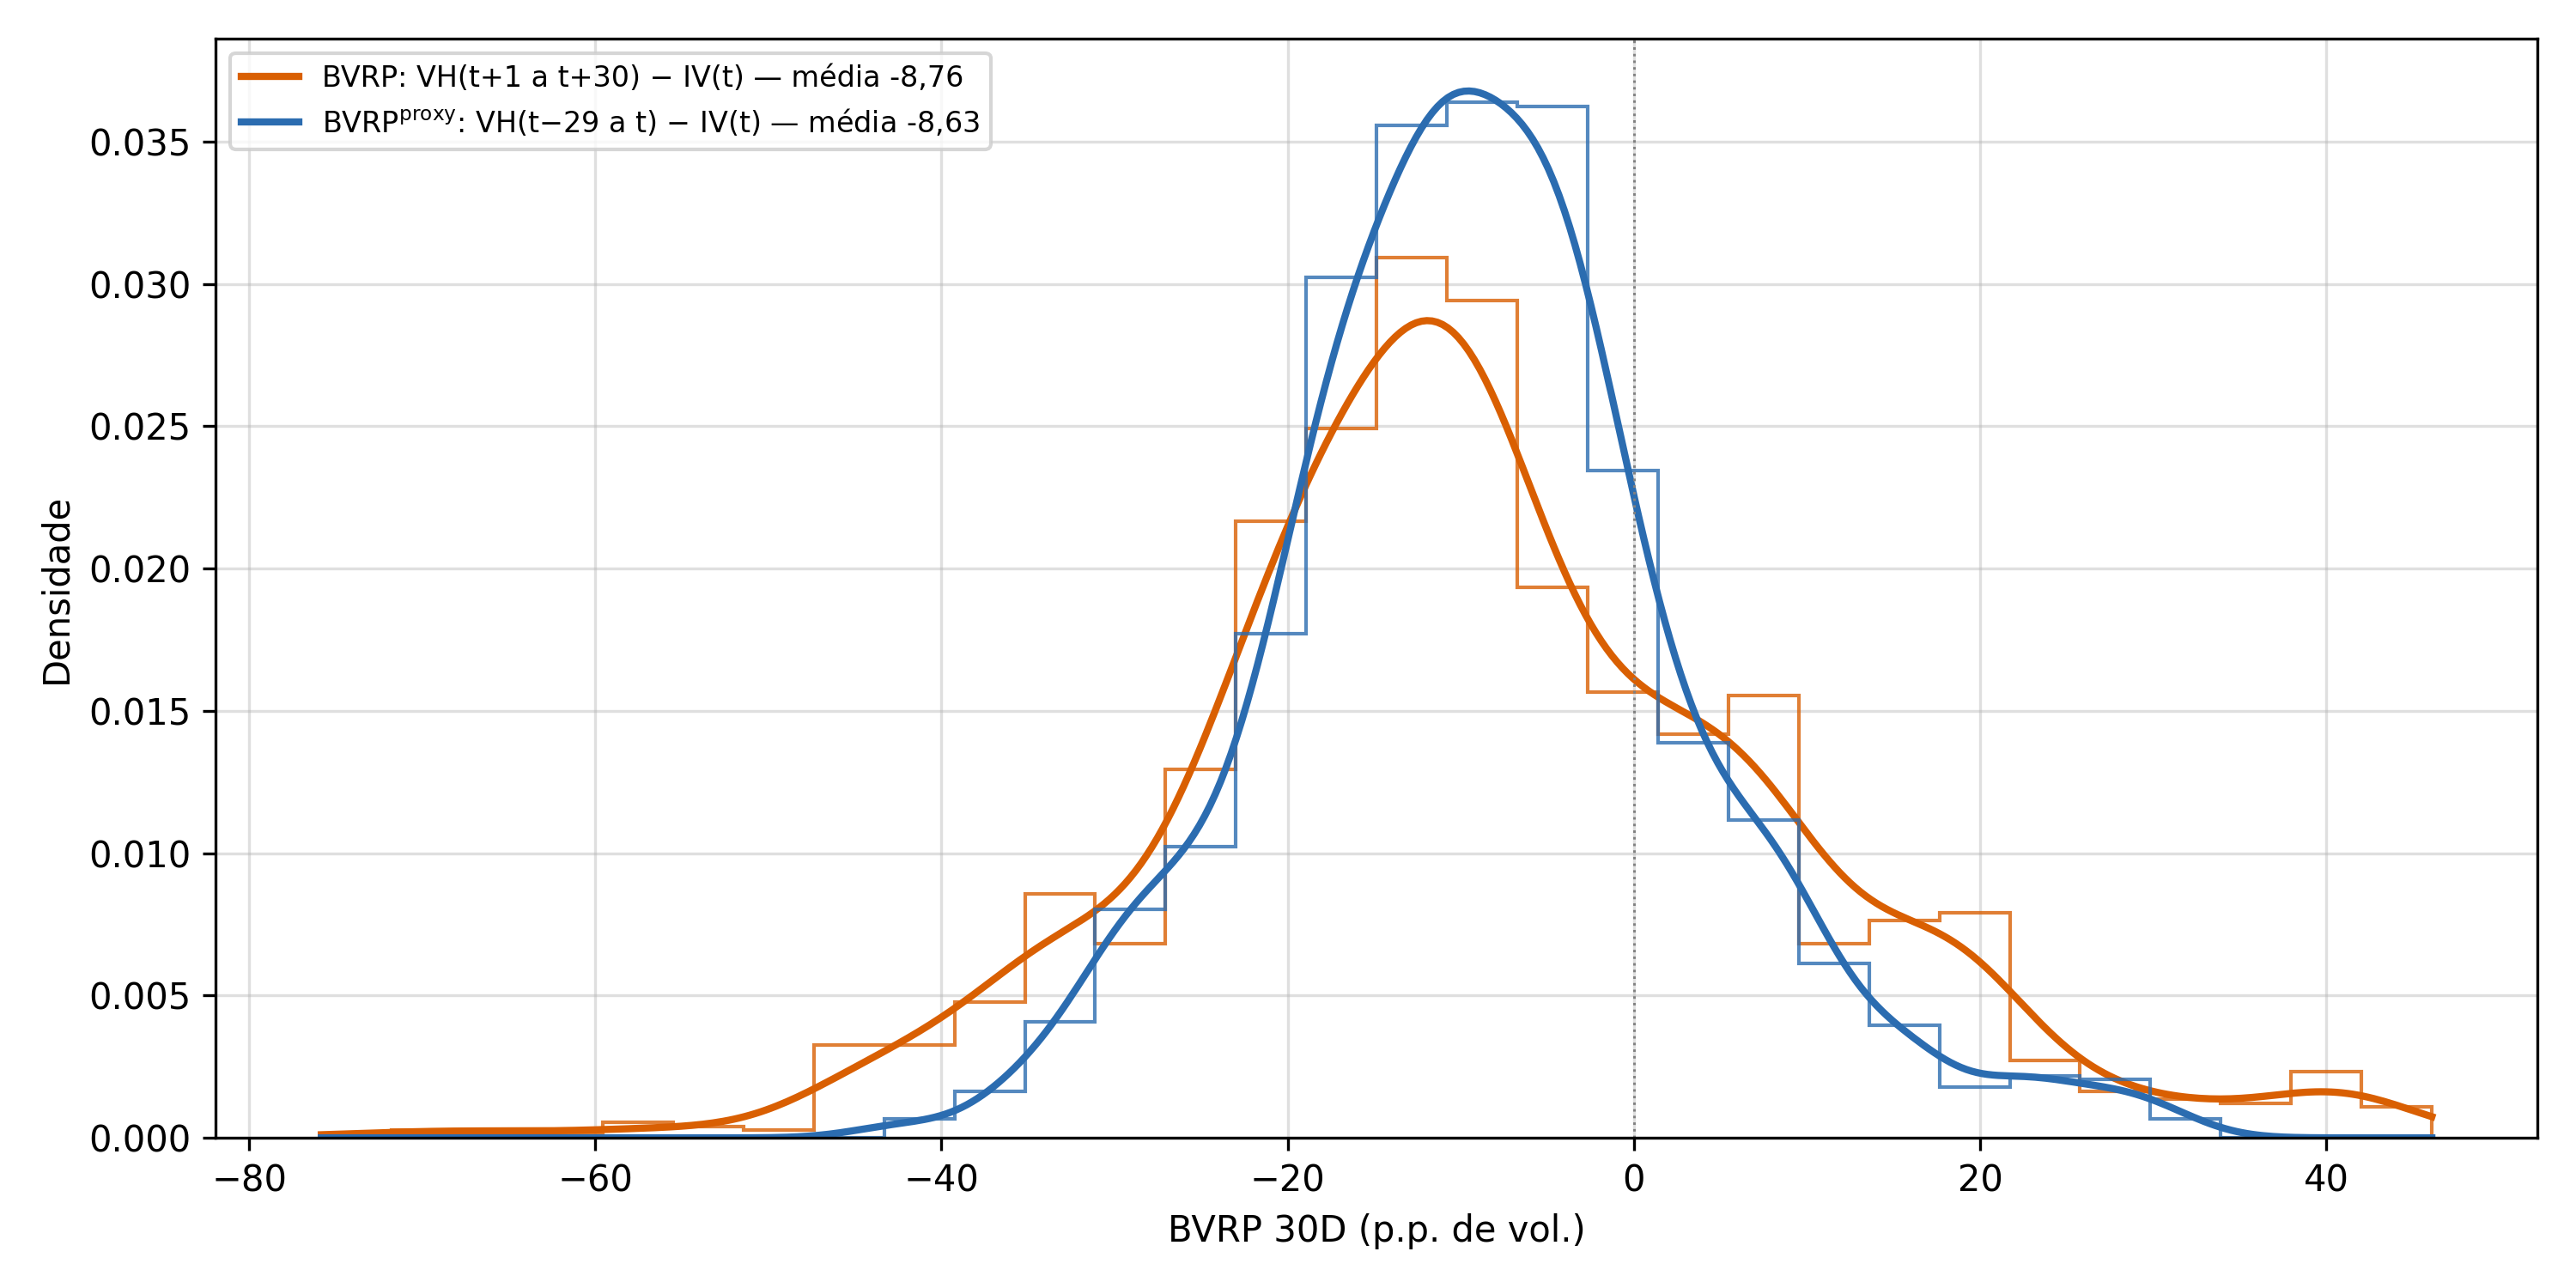
\includegraphics[width=0.75\linewidth]{figs/dados/vrp_histogram_kde.png}
    \caption{Distribuição empírica do prêmio de risco de volatilidade do Bitcoin: BVRP e $\text{BVRP}^{\text{proxy}}$ (histogramas e densidades de núcleo).}
    \label{fig:dados-histograma}
\end{figure}
}{}

As duas distribuições são unimodais, com moda em torno de $-12$ p.p. no BVRP e
de $-10$ p.p. na proxy, consistente com as médias negativas e com o predomínio
de datas em que a volatilidade implícita supera a histórica. Ambas apresentam
assimetria positiva ($0{,}24$ e $0{,}38$) e excesso de curtose moderado
($0{,}73$ e $0{,}67$), afastando-se da hipótese de normalidade. O BVRP tem
caudas mais longas, porque a volatilidade histórica dos 30 dias seguintes reage
a choques que a IV de $t$ não antecipa. Sem a correção de março de 2023, as
datas de abril de 2023 formariam, na proxy, uma moda local espúria na cauda
positiva, perto de $+27$ p.p.

A cauda direita reúne uma minoria de observações positivas, correspondentes a
episódios de estresse agudo em que a volatilidade histórica supera
inesperadamente a implícita. Esses episódios ocorrem durante choques abruptos
de mercado, quando a magnitude das oscilações de preço supera as expectativas
incorporadas nos prêmios de opções. Com dados diários, não é possível separar,
nesses episódios, os movimentos contínuos dos descontínuos (saltos): essa
decomposição exigiria dados intradiários, indisponíveis nesta dissertação.

% =========================================================
\section{Regimes de volatilidade e subperíodos}
\label{sec:dados-regimes}

Ao contrário da distribuição do prêmio, a distribuição da volatilidade
histórica de 30 dias é bimodal, e a bimodalidade costuma ser evidência de dois
regimes: as modas associam-se às médias dos regimes, e a antimoda separa os
dois. A Figura~\ref{fig:dados-vh-bimodal} mostra o histograma da volatilidade
histórica, em escala logarítmica, na primeira janela de estimação (23/04/2021 a
22/04/2023), com uma mistura de duas normais ajustada aos dados. O componente
de baixa volatilidade tem média de $31{,}2\%$ a.a. e peso de $0{,}08$; o de
alta, média de $66{,}7\%$ a.a. O ponto em que os dois componentes passam a ter
a mesma probabilidade a posteriori, $37{,}3\%$ a.a., coincide com a antimoda da
densidade de núcleo ($37{,}5\%$ a.a.) e define o corte entre o regime de baixa
volatilidade e o regime de alta volatilidade. Como o corte usa apenas a
primeira janela, nenhuma data é classificada com informação posterior a ela
(Capítulo~\ref{chap:metodologia}). A bimodalidade perde nitidez com a queda da
volatilidade do Bitcoin a partir de 2025: reestimada em janela expansiva, a
mistura troca de solução entre fevereiro e julho de 2025, e o corte passa a
oscilar.

\IfFileExists{figs/dados/vh_bimodalidade.png}{
\begin{figure}[H]
    \centering
    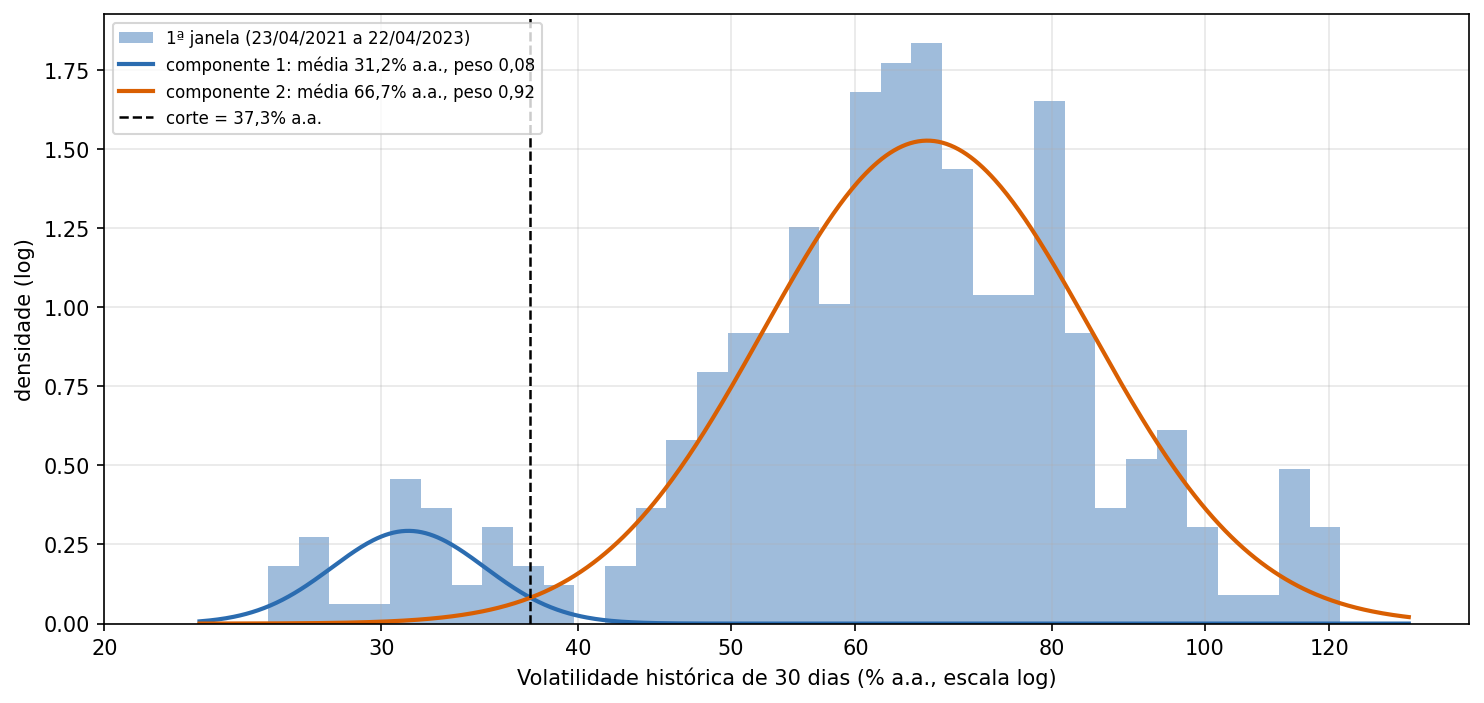
\includegraphics[width=0.85\linewidth]{figs/dados/vh_bimodalidade.png}
    \caption{Volatilidade histórica de 30 dias na primeira janela de estimação (23/04/2021 a 22/04/2023), em escala logarítmica: histograma, mistura de duas normais e corte de $37{,}3\%$ a.a. entre os regimes de baixa e de alta volatilidade.}
    \label{fig:dados-vh-bimodal}
\end{figure}
}{}

O prêmio difere entre os regimes, e a direção da diferença depende da versão.
Como $\text{BVRP} = \text{VH} - \text{IV}$, prêmio maior corresponde a BVRP mais
negativo; \citet{almeida2024cryptoVRP}, que medem o prêmio pela variância
neutra ao risco menos a física, usam o sinal oposto. Na proxy, o prêmio é maior
no regime de baixa volatilidade: a média é de $-13{,}56$ p.p. nas 394 datas
desse regime e de $-7{,}26$ p.p. nas 1.412 do regime de alta. A diferença, de
$6{,}30$ p.p., é estimada por MQO da proxy numa variável indicadora do regime
de alta, com erro-padrão de Newey--West de 31 defasagens ($2{,}10$;
$p = 0{,}003$). É o padrão que \citet{almeida2024cryptoVRP} encontram com dois
regimes obtidos de outra forma e com a variância realizada dos 27 dias
anteriores, também retrospectiva. No BVRP, a diferença se inverte: a média é de
$+2{,}00$ p.p. no regime de baixa e de $-11{,}77$ p.p. no de alta (diferença de
$-13{,}77$ p.p., com erro-padrão de $3{,}55$; $p < 0{,}001$). A inversão vem da
volatilidade histórica. No regime de baixa, a VH dos 30 dias anteriores tem
média de $30{,}7\%$ a.a., a IV, de $44{,}2\%$, e a VH dos 30 dias seguintes, de
$46{,}2\%$: a IV supera a volatilidade recente, mas não a que se realiza em
seguida. A proxy, que compara a IV com a VH passada, registra um prêmio grande;
o BVRP, que a compara com a VH futura, não. Parte da diferença na proxy é, além
disso, mecânica: o regime é definido pela mesma $\text{VH}_{t-29:t}$ que entra
na proxy, e, no regime de baixa, a proxy é negativa em todas as datas.

Para avaliar a heterogeneidade temporal do prêmio, a
Figura~\ref{fig:dados-boxplot-anual} agrupa a amostra por ano e apresenta a
distribuição do BVRP e da proxy em cada subperíodo.

\IfFileExists{figs/dados/vrp_boxplot.png}{
\begin{figure}[H]
    \centering
    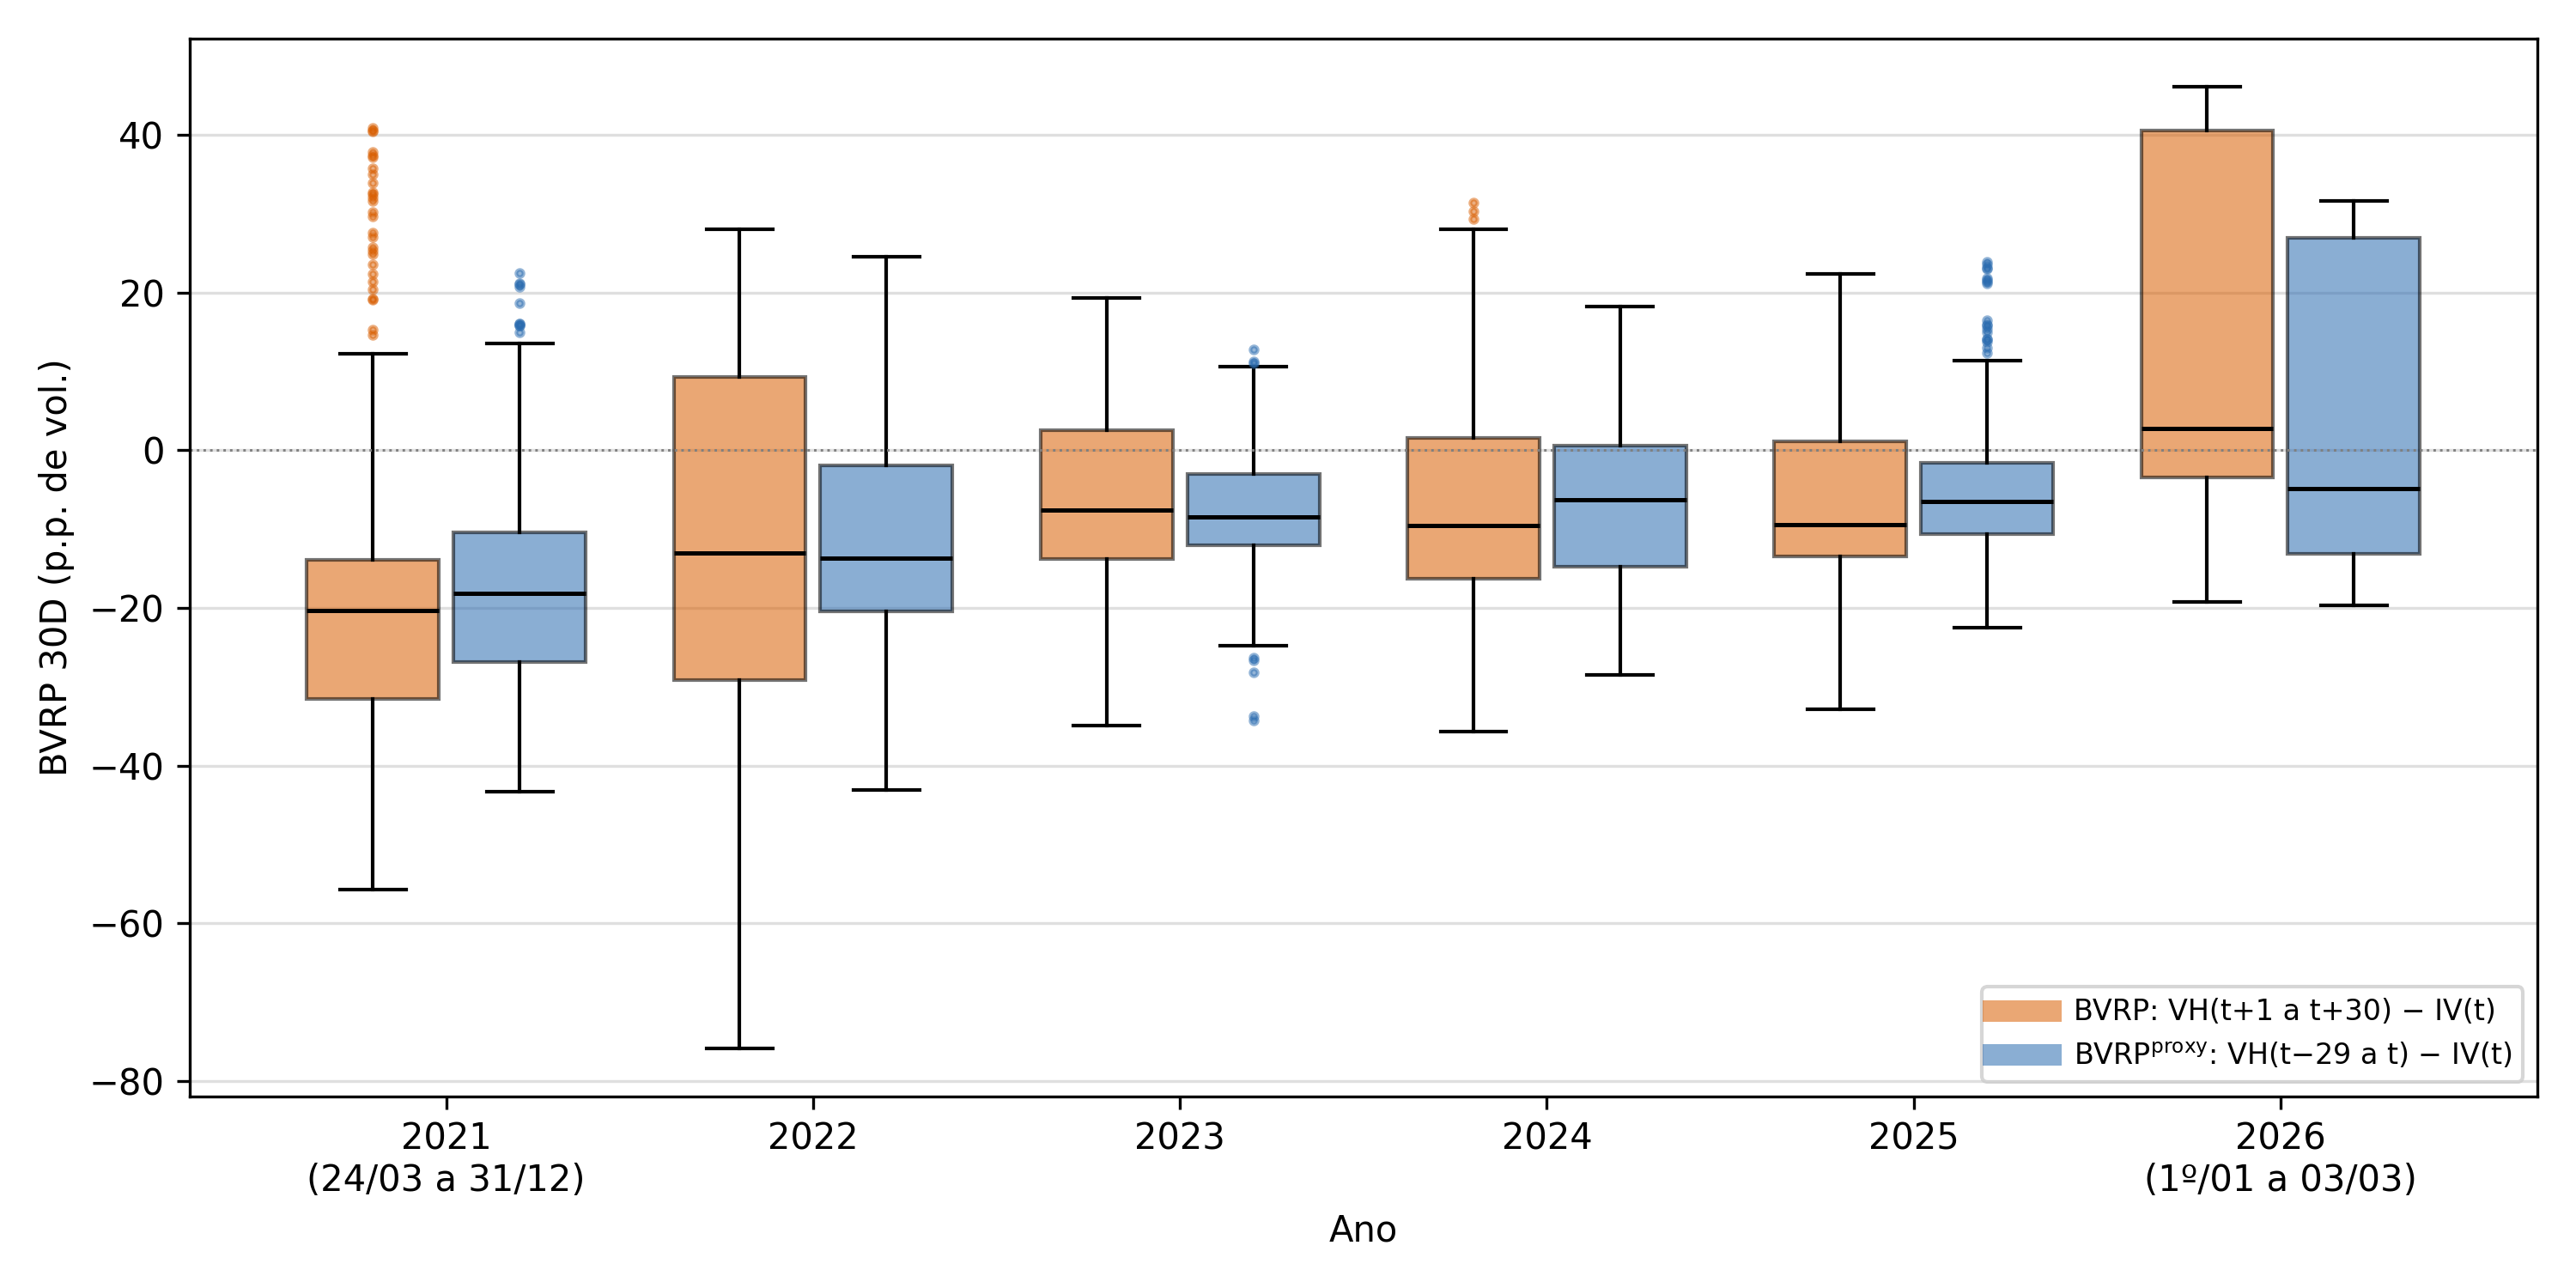
\includegraphics[width=0.85\linewidth]{figs/dados/vrp_boxplot.png}
    \caption{Distribuição anual do prêmio de risco de volatilidade do Bitcoin: BVRP e $\text{BVRP}^{\text{proxy}}$. O primeiro e o último anos estão incompletos: 2021 cobre de 24/03 a 31/12/2021 ($N = 283$), e 2026, apenas de 1º/01 a 03/03/2026 ($N = 62$); a distribuição de 2026 não é comparável à dos anos completos.}
    \label{fig:dados-boxplot-anual}
\end{figure}
}{}

Os resultados indicam que o prêmio de risco de volatilidade não é homogêneo ao
longo do tempo. Nos anos completos, a mediana do BVRP é negativa em todos os
anos e atenua-se ao longo do período, passando de $-20{,}3$ p.p. em 2021 para
cerca de $-9{,}5$ p.p. em 2024 e 2025; a proxy segue o mesmo padrão (de
$-18{,}1$ para $-6{,}5$ p.p.). A dispersão, contudo, não acompanha essa
tendência de forma monotônica. O ano de 2022 exibe a maior variabilidade do
BVRP entre os anos completos (amplitude interquartílica de $38{,}4$ p.p.,
contra $14{,}6$ a $17{,}8$ p.p. nos demais), refletindo a sequência de crises do
período. Na proxy, 2023 e 2025 apresentam as distribuições mais comprimidas
(amplitude interquartílica de $9{,}1$ p.p.), e 2024, dispersão novamente
elevada ($15{,}4$ p.p.), no primeiro ano após a aprovação dos ETFs à vista,
em janeiro de 2024. O início de
2026 concentra um episódio agudo de estresse, visível como um pico pronunciado
ao final da série temporal (Figura~\ref{fig:dados-series}), e a mediana do
BVRP chega a $+2{,}7$ p.p.; com apenas 62 observações, porém, esse período não
é comparável aos anos completos. Essa heterogeneidade sugere que modelos com
parâmetros constantes podem ser insuficientes para capturar plenamente a
dinâmica do BVRP, justificando a adoção de abordagens que permitam variação
temporal e efeitos de regime nos capítulos subsequentes.

% =========================================================
\section{Relações iniciais entre prêmio de risco de volatilidade e retornos}
\label{sec:dados-bvrp-retornos}

Por fim, esta seção examina a relação exploratória entre o prêmio de risco de
volatilidade do Bitcoin e os retornos futuros do ativo. A
Figura~\ref{fig:dados-bvrp-retorno-30d} apresenta o gráfico de dispersão entre a
$\text{BVRP}^{\text{proxy}}$ observada em $t$ e o retorno acumulado do Bitcoin
nos 30 dias seguintes, juntamente com a reta de MQO. O horizonte de 30 dias
coincide com o do prêmio. A figura usa a proxy, e não o BVRP, porque o BVRP de
$t$ é calculado com os mesmos retornos de $t+1$ a $t+30$ que formam o retorno
futuro, e a relação entre os dois seria em parte mecânica.

\IfFileExists{figs/dados/vrp_vs_return_30d.png}{
\begin{figure}[H]
    \centering
    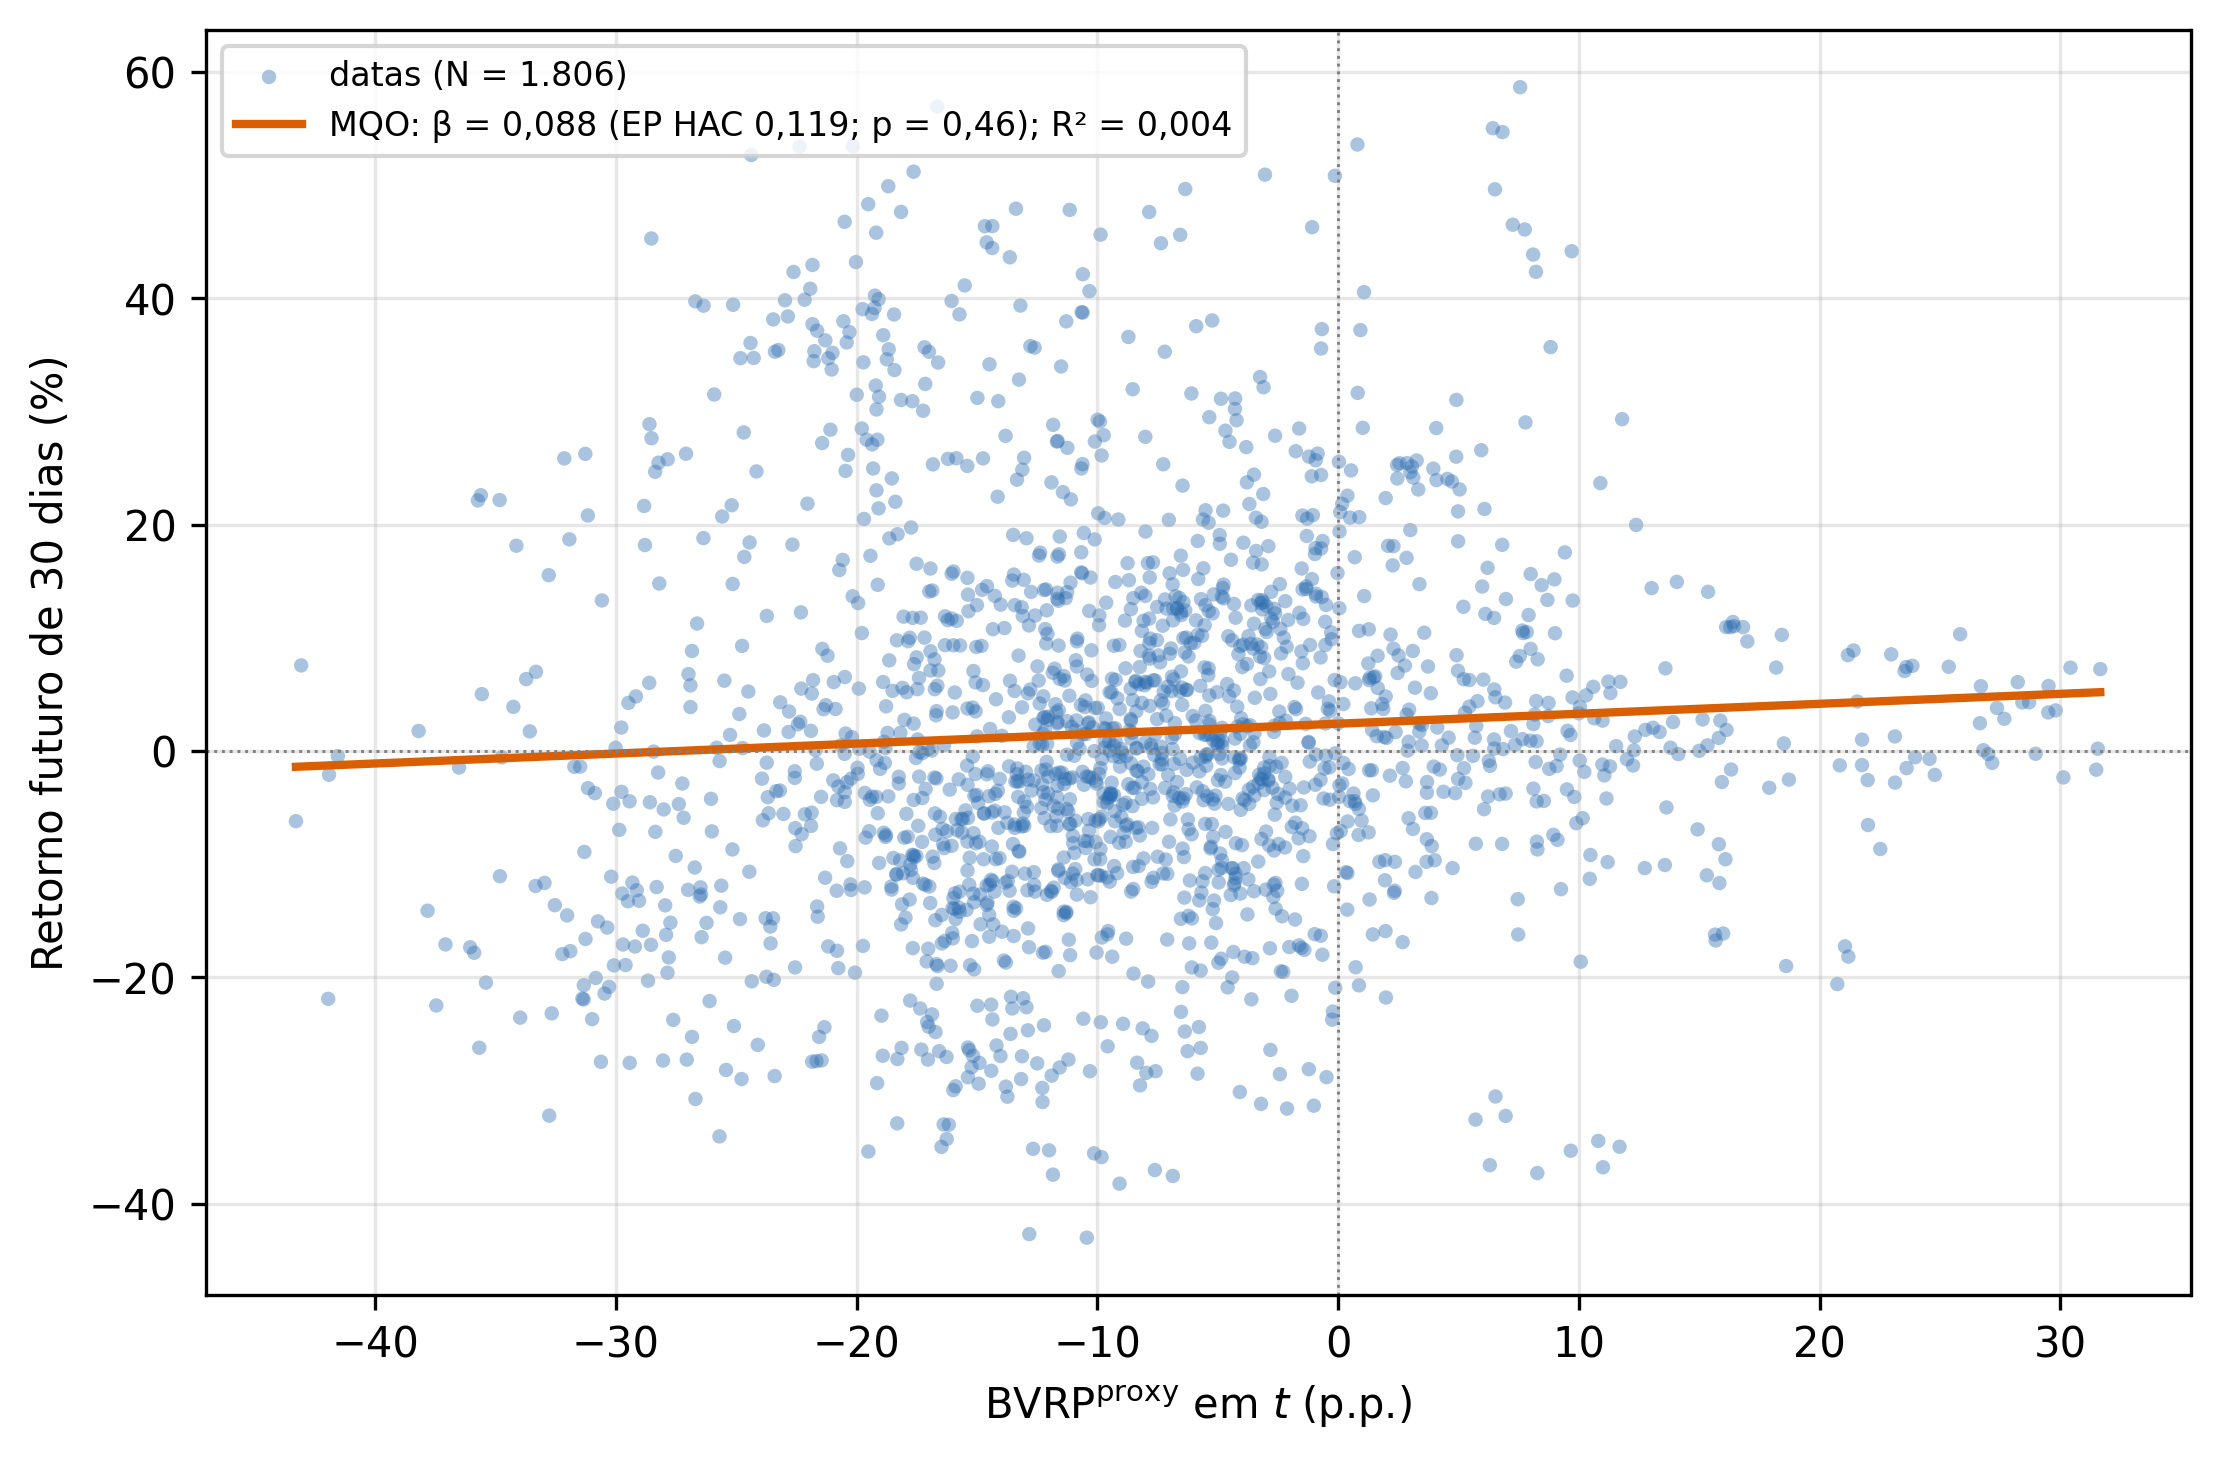
\includegraphics[width=0.75\linewidth]{figs/dados/vrp_vs_return_30d.png}
    \caption{Relação exploratória entre a $\text{BVRP}^{\text{proxy}}$ em $t$ e o
    retorno do Bitcoin nos 30 dias seguintes ($N = 1.806$). Reta de MQO, com
    erro-padrão de Newey--West de 31 defasagens.}
    \label{fig:dados-bvrp-retorno-30d}
\end{figure}
}{}

O gráfico não evidencia associação linear relevante entre o prêmio e os
retornos futuros: o coeficiente da reta é de $0{,}088$ (erro-padrão HAC de
$0{,}119$; valor-$p$ de $0{,}46$), o $R^2$ é de $0{,}004$ e a correlação, de
$0{,}06$, e a nuvem de pontos dispersa-se amplamente em torno de uma reta quase
horizontal. Essa ausência de relação linear na análise exploratória antecipa,
de forma preliminar, o resultado central do Capítulo~\ref{chap:retornos_linear},
em que o regressor é o BVRP previsto, e não a proxy, e nenhum horizonte é
significante depois das correções para o regressor gerado e para as
comparações múltiplas. A dispersão
elevada indica que, se o prêmio de risco de volatilidade carrega conteúdo
informacional sobre o desempenho futuro do Bitcoin, esse conteúdo não se
manifesta em uma relação linear simples --- motivando as abordagens não
lineares e condicionais desenvolvidas nos capítulos subsequentes.
